%% BioMed_Central_Tex_Template_v1.06
%%                                      %
%  bmc_article.tex            ver: 1.06 %
%                                       %

%%IMPORTANT: do not delete the first line of this template

%%%%%%%%%%%%%%%%%%%%%%%%%%%%%%%%%%%%%%%%%
%%                                     %%
%%  LaTeX template for BioVis 2014  %%
%%      article submissions     %%
%%          adapted from BMC    %%
%%          <8 Jan 2014>              %%
%% Liz Marai (g.elisabeta.marai@gmail.com) %%
%%                                     %%
%%%%%%%%%%%%%%%%%%%%%%%%%%%%%%%%%%%%%%%%%


%%%%%%%%%%%%%%%%%%%%%%%%%%%%%%%%%%%%%%%%%%%%%%%%%%%%%%%%%%%%%%%%%%%%%
%%                                                                 %%
%%%%%%%%%%%%%%%%%%%%%%%%%%%%%%%%%%%%%%%%%%%%%%%%%%%%%%%%%%%%%%%%%%%%%

%%% additional documentclass options:
%  [doublespacing]
%  [linenumbers]   - put the line numbers on margins

%%% loading packages, author definitions

\documentclass[twocolumn]{bmcart}% uncomment this for twocolumn layout 



%%% Load packages
%\usepackage{amsthm,amsmath}
%\RequirePackage{natbib}
%\RequirePackage{hyperref}
\usepackage[utf8]{inputenc} %unicode support
%\usepackage[applemac]{inputenc} %applemac support if unicode package fails
%\usepackage[latin1]{inputenc} %UNIX support if unicode package fails
\usepackage{graphicx}

%%%%%%%%%%%%%%%%%%%%%%%%%%%%%%%%%%%%%%%%%%%%%%%%%
%%                                             %%
%%  If you wish to display your graphics for   %%
%%  your own use using includegraphic or       %%
%%  includegraphics, then comment out the      %%
%%  following two lines of code.               %%
%%%%%%%%%%%%%%%%%%%%%%%%%%%%%%%%%%%%%%%%%%%%%%%%%


%\def\includegraphic{}
%\def\includegraphics{}



%%% Put your definitions there:
\startlocaldefs
\endlocaldefs


%%% Begin ...
\begin{document}

%%% Start of article front matter
\begin{frontmatter}

\begin{fmbox}
\dochead{Research}

%%%%%%%%%%%%%%%%%%%%%%%%%%%%%%%%%%%%%%%%%%%%%%
%%                                          %%
%% Enter the title of your article here     %%
%%                                          %%
%%%%%%%%%%%%%%%%%%%%%%%%%%%%%%%%%%%%%%%%%%%%%%

\title{Comparative Visualization of Protein Secondary Structures}

%%%%%%%%%%%%%%%%%%%%%%%%%%%%%%%%%%%%%%%%%%%%%%
%%                                          %%
%% Do not enter the authors here for        %%
%%  a double-blind review. Otherwise        %%
%% specify information, if available,       %%
%% in the form:                             %%
%%   <key>={<id1>,<id2>}                    %%
%%   <key>=                                 %%
%% Comment or delete the keys which are     %%
%% not used. Repeat \author command as much %%
%% as required.                             %%
%%                                          %%
%%%%%%%%%%%%%%%%%%%%%%%%%%%%%%%%%%%%%%%%%%%%%%
\author[
     addressref={aff1},
  % noteref={n2},
   email={lucia.koc@gmail.com}
]{\inits{LK}\fnm{Lucia} \snm{Kocincov\'{a}}}
\author[
   addressref={aff1},                   % id's of addresses, e.g. {aff1,aff2}
   %corref={aff1},                       % id of corresponding address, if any
   %noteref={n1},                        % id's of article notes, if any
  email={jaresova@mail.muni.cz}   % email address
]{\inits{MJ}\fnm{Miroslava} \snm{Jare\v{s}ov\'{a}}}
\author[
   addressref={aff1,aff2},                   % id's of addresses, e.g. {aff1,aff2}
   %corref={aff1},                       % id of corresponding address, if any
   %noteref={n1},                        % id's of article notes, if any
  email={xbyska@fi.muni.cz}   % email address
]{\inits{JB}\fnm{Jan} \snm{By\v{s}ka}}
\author[
   addressref={aff2},                   % id's of addresses, e.g. {aff1,aff2}
   %corref={aff1},                       % id of corresponding address, if any
   %noteref={n1},                        % id's of article notes, if any
  email={julius.parulek@uib.no}   % email address
]{\inits{JP}\fnm{J\'{u}lius} \snm{Parulek}}
\author[
   addressref={aff2},                   % id's of addresses, e.g. {aff1,aff2}
   %corref={aff1},                       % id of corresponding address, if any
   %noteref={n1},                        % id's of article notes, if any
  email={Helwig.Hauser@uib.no}   % email address
]{\inits{HH}\fnm{Helwig} \snm{Hauser}}
\author[
   addressref={aff1},                   % id's of addresses, e.g. {aff1,aff2}
   %corref={aff1},                       % id of corresponding address, if any
   %noteref={n1},                        % id's of article notes, if any
  email={kozlikova@fi.muni.cz}   % email address
]{\inits{BK}\fnm{Barbora} \snm{Kozl\'{i}kov\'{a}}}


%%%%%%%%%%%%%%%%%%%%%%%%%%%%%%%%%%%%%%%%%%%%%%
%%                                          %%
%% Enter the authors' addresses here        %%
%%                                          %%
%% Repeat \address commands as much as      %%
%% required.                                %%
%%                                          %%
%%%%%%%%%%%%%%%%%%%%%%%%%%%%%%%%%%%%%%%%%%%%%%

\address[id=aff1]{%                           % unique id
  \orgname{Masaryk University}, % university, etc
 % \postcode{60200}                                % post or zip code
  \city{Brno},                              % city
  \cny{Czech Republic}                                    % country
}
\address[id=aff2]{%                           % unique id
  \orgname{University of Bergen}, % university, etc
%  \street{210 South Bouquet},                     %
  %\postcode{15260}                                % post or zip code
  %\city{Bergen},                              % city
  \cny{Norway}                                    % country
}


%%%%%%%%%%%%%%%%%%%%%%%%%%%%%%%%%%%%%%%%%%%%%%
%%                                          %%
%% Enter short notes here                   %%
%%                                          %%
%% Short notes will be after addresses      %%
%% on first page.                           %%
%%                                          %%
%%%%%%%%%%%%%%%%%%%%%%%%%%%%%%%%%%%%%%%%%%%%%%

\begin{artnotes}
%\note{Sample of title note}     % note to the article
%\note[id=n1]{Equal contributor} % note, connected to author
%\note[id=n2]{Equal contributor} % note, connected to author
%\note[id=n3]{Equal contributor} % note, connected to author
%\note[id=n4]{Project leader and equal contributor} % note, connected to author
\end{artnotes}

\end{fmbox}% comment this for two column layout

%%%%%%%%%%%%%%%%%%%%%%%%%%%%%%%%%%%%%%%%%%%%%%
%%                                          %%
%% The Abstract begins here                 %%
%%                                          %%
%% Please refer to the Instructions for     %%
%% authors on http://www.biomedcentral.com  %%
%% and include the section headings         %%
%% accordingly for your article type.       %%
%%                                          %%
%%%%%%%%%%%%%%%%%%%%%%%%%%%%%%%%%%%%%%%%%%%%%%

\begin{abstractbox}

\begin{abstract} % abstract, must be under 350 words
%\parttitle{First part title} %if any
%Text for this section.
  

\parttitle{Background} 
Protein function is determined by many factors, namely by its constitution, spatial arrangement, and dynamic behavior. 
Studying these factors helps the biochemists and biologists to better understand the protein behavior and to design proteins with modified properties.
One of the most common approaches to these studies is to compare the protein structure with other molecules and to reveal similarities and differences in their polypeptide chains.

%Visual comparison of molecular structures could provide domain experts with an important information about the similarities and differences in their protein chains. Information about the amino acids (AA) is typically conveyed via secondary structures or as a 1D sequence of AA forming the protein chain. 

\parttitle{Results} 
We support the comparison process by proposing a new visualization technique that bridges the gap between traditionally used 1D and 3D representations.
By introducing the information about mutual positions of protein chains into the 1D sequential representation the users are able to observe the spatial differences between the proteins without any occlusion commonly present in 3D view.
Our representation is designed to serve namely for comparison of multiple proteins or a set of time steps of molecular dynamics simulation.
%It aims to enhance the 1D sequential representation by adding parameters derived from geometry of secondary structures.
%The core of our technique is based on unrolling the protein chain to a line while maintaining the mutual orientation of secondary structures as well as their lengths. 
%Then the user can explore in detail structures of interest, which are visually compared via superimposition and juxtaposition techniques. 

\parttitle{Conclusions}  
The novel representation is demonstrated on two case studies.
The first study aims to compare a set of proteins from the family of cytochromes P450 where the position of the secondary structures has a significant impact on the substrate channeling.
The second study focuses on the protein flexibility when by comparing a set of time steps our representation helps to reveal the most dynamically changing parts of the protein chain.

%\parttitle{Second part title} %if any
%Text for this section.
\end{abstract}

%%%%%%%%%%%%%%%%%%%%%%%%%%%%%%%%%%%%%%%%%%%%%%
%%                                          %%
%% The keywords begin here                  %%
%%                                          %%
%% Put each keyword in separate \kwd{}.     %%
%%                                          %%
%%%%%%%%%%%%%%%%%%%%%%%%%%%%%%%%%%%%%%%%%%%%%%

\begin{keyword}
\kwd{Molecular Visualization}
\kwd{Molecular Sequence Analysis}
\kwd{Molecular Structure and Function}
\end{keyword}

% MSC classifications codes, if any
%\begin{keyword}[class=AMS]
%\kwd[Primary ]{}
%\kwd{}
%\kwd[; secondary ]{}
%\end{keyword}

\end{abstractbox}
%
%\end{fmbox}% uncomment this for twcolumn layout

\end{frontmatter}

%%%%%%%%%%%%%%%%%%%%%%%%%%%%%%%%%%%%%%%%%%%%%%
%%                                          %%
%% The Main Body begins here                %%
%%                                          %%
%% Please refer to the instructions for     %%
%% authors on:                              %%
%% http://www.biomedcentral.com/info/authors%%
%% and include the section headings         %%
%% accordingly for your article type.       %%
%%                                          %%
%% See the Results and Discussion section   %%
%% for details on how to create sub-sections%%
%%                                          %%
%% use \cite{...} to cite references        %%
%%  \cite{koon} and                         %%
%%  \cite{oreg,khar,zvai,xjon,schn,pond}    %%
%%  \nocite{smith,marg,hunn,advi,koha,mouse}%%
%%                                          %%
%%%%%%%%%%%%%%%%%%%%%%%%%%%%%%%%%%%%%%%%%%%%%%

%%%%%%%%%%%%%%%%%%%%%%%%% start of article main body
% <put your article body there>

%%%%%%%%%%%%%%%%
%% Background %%
%%
\section*{Background}
Studying the structure of proteins has been in the scope of researchers for many decades, namely because of their importance in all living cells. 
Better understanding of their constitution and behavior helps to understand and control their function and properties.

Protein structure consists of a polypeptide chain of amino acids, which is unique for each type of protein. 
The chain is folded into a spatial conformation that exhibits specific patterns, called secondary structures.
Among these structures belong so called alpha-helices and beta-sheets. 
The amino acids forming these secondary structures maintain their shape thanks to weak hydrogen bonds between them.
Visual representation of the protein consisting of secondary structures is denoted as cartoon or ribbon (see Figure~\ref{fig:aquaria} left).
This highly abstracted visualization omits individual atoms of the protein and highlights only the protein backbone represented by the secondary structures.
Such a representation is very popular by researchers because of its balanced tradeoff between the level of abstractness and conveying the spatial arrangement of the chain.

\begin{figure*}[th]
  \centering
  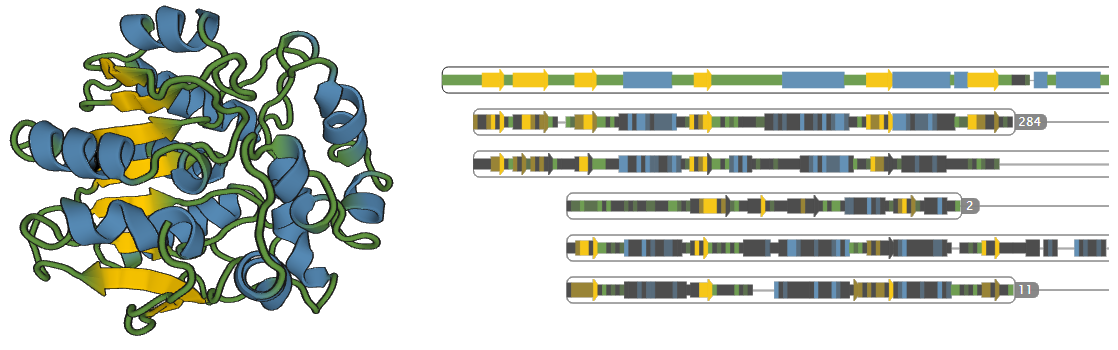
\includegraphics[width=0.9\textwidth]{pics/aquaria.png}
  \caption{Left -- cartoon representation of the DhaA haloalkane dehalogenase (PDB ID 1CQW). Right -- part of the sequential representation of DhaA along with the information about secondary structures and several other structures sequentially aligned to DhaA. Images generated using the Aquaria tool by O'Donoghue et al.~\cite{odonoghue2015}.}
  \label{fig:aquaria}
\end{figure*}

When comparing several protein structures, e.g., when searching for similar structures in order to get the information about an unknown protein, there are several existing algorithms for aligning such structures~\cite{dali,Shindyalov1998,ssap,tmalign,promals3d}.
These algorithms are aligning the whole structures (structure alignment) or are parsing the sequence of amino acids and searching for corresponding patterns (sequence alignment). 
The results of these alignments are traditionally presented in a form of color-coded one-dimensional sequential information (see Figure~\ref{fig:align}).

\begin{figure}[bh]
  \centering
  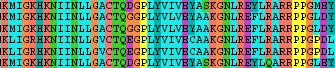
\includegraphics[width=0.9\columnwidth]{pics/align.png}
  \caption{Example of the sequence alignment visualization.}
  \label{fig:align}
\end{figure}

Each row represents one protein structure and the user can observe both similarities and differences between protein chains by exploring the columns.
Some methods equip the sequence with the information about secondary structures (see Figure~\ref{fig:aquaria} right).
However, all of them lack the mutual spatial orientation of the secondary structures of the aligned structures.
This information is crucial in many cases, namely when exploring the protein inner void space that plays a significant role in protein reactivity with other molecules.
This void space is determined by the surrounding amino acids, i.e., secondary structures. 
Therefore, the changes in the spatial position of secondary structures directly influence the volume and shape of the void space.

The mutual spatial arrangement of the secondary structures can be easily observed in a 3D view. 
However, for comparison of multiple proteins, such a representation is very limited with respect to its scalability.
In other words, due to the occlusion problems, the spatial representation is suitable for comparison of only few structures. 
Figure~\ref{fig:many} demonstrates the case when six similar proteins are aligned.
Even with such a small number of molecules it is hard to perceive the differences in the secondary structure positions.

%One of the most important ones is the presence of a void space inside the protein which directly influences the protein reactivity with a small ligand. 
%The interaction with the ligand occurs often deeply inside the protein and the 

\begin{figure}[th]
  \centering
  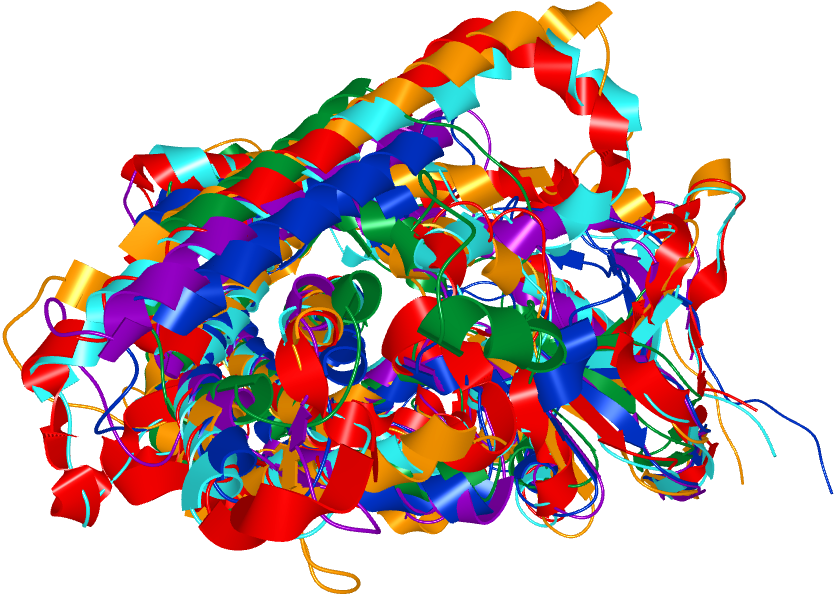
\includegraphics[width=0.9\columnwidth]{pics/many.png}
  \caption{Spatial representation of structure alignment of six proteins from the cytochrome P450 family which have very similar constitution.}
  \label{fig:many}
\end{figure}

To overcome the problems of the lack of mutual arrangement of the compared protein in the sequential representation and problems with occlusion in the spatial view, we propose a new method designed to serve as a tool for comparison of multiple structures and intuitive exploration of their spatial differences.
It benefits from the sequential information which consists of individual secondary structures, and when comparing this sequence with other proteins, it encodes the mutual spatial arrangement of the secondary structures of the aligned proteins.
In consequence, the user can observe this arrangement without occlusion issues present in the 3D view.
Our solution also utilizes the fact that the domain experts are well accustomed with the sequential representation as well as with secondary structures and their cartoon representation. 
Therefore, our proposed visualization is interactively linked with the 3D view.
Selection of interesting secondary structures in the novel representation is directly projected to this spatial view. 

\begin{figure*}[t]
  \centering
  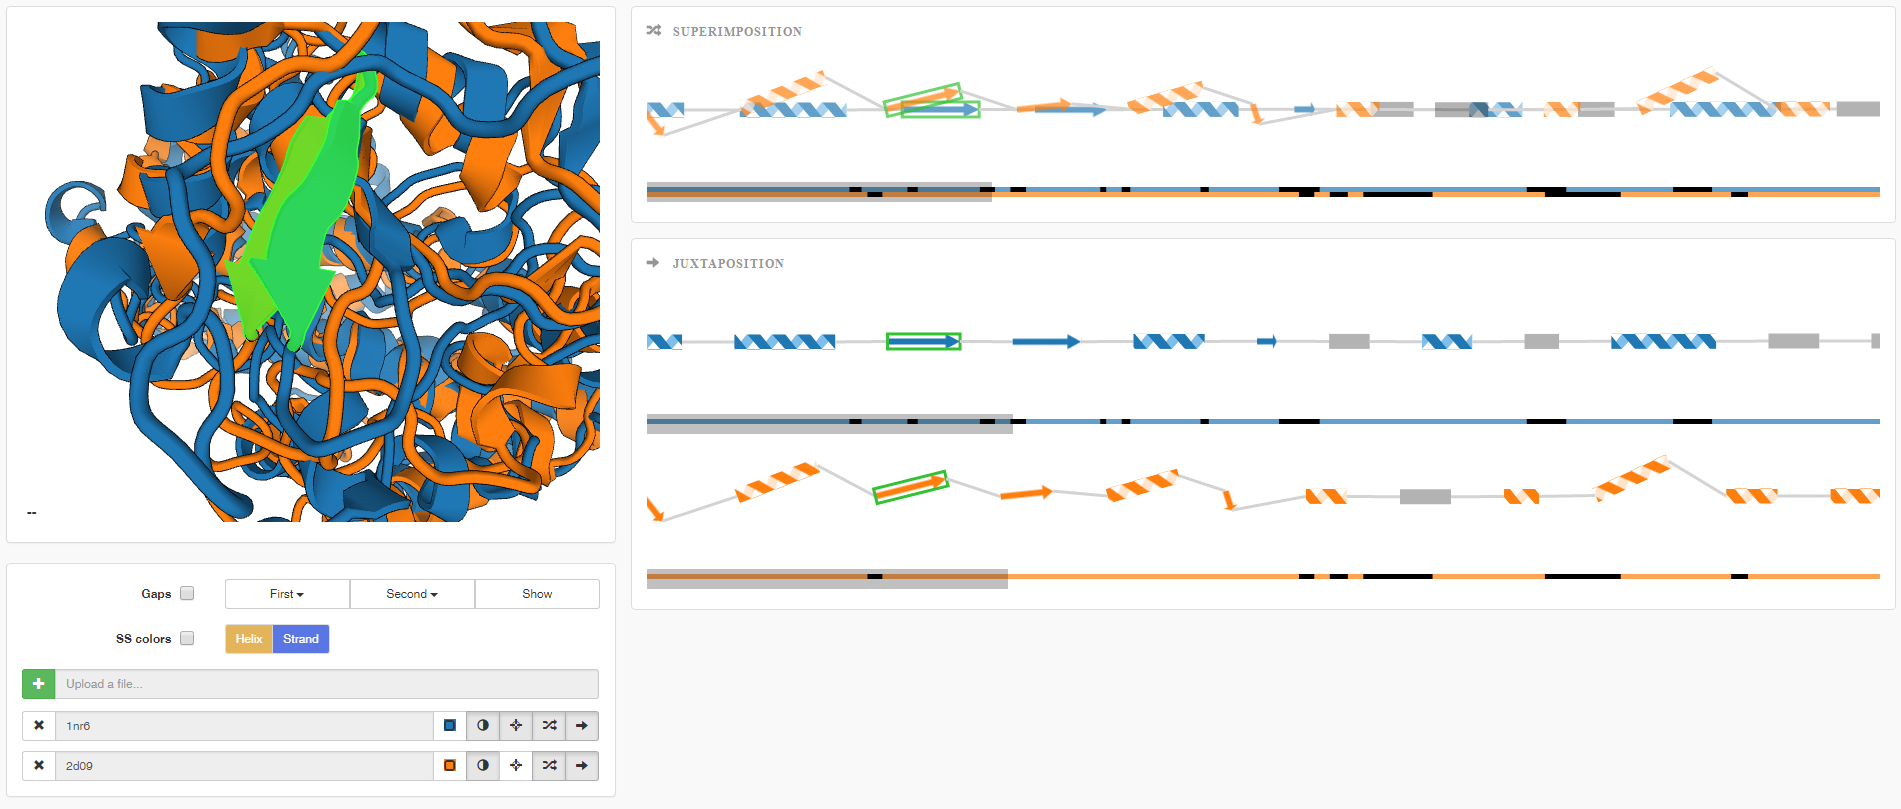
\includegraphics[width=0.9\textwidth]{pics/flattening_design2.png}
  \caption{Overview of the proposed system. Top left part contains the 3D visualization window integrating the PV viewer~\cite{biasini2014}. The right part contains our proposed visualization methods serving for comparison of two or more protein chains. It consists of superimposed and juxtaposed views. Bottom left part contains the user interface.}
  \label{fig:design}
\end{figure*}

\subsection*{Related Work}

An exhaustive and comprehensive review on the methods, tools and applications of 2D molecular graphics was presented by Zhou and Shang \cite{Zhou2009}. 
The review covers numerous approaches to generation and drawing of chemical structures, protein topology representation and schematic layout of molecular interactions.
The evaluation of common visualization techniques in context of their dimensionality is covered in the work of Heinrich \cite{Heinrich2014}.
The expected benefits and drawbacks of using manifold visualizations when solving particular tasks are discussed in order to propose ideas how to improve those techniques.

According to Stivala \cite{Stivala2011}, there are four systems specializing in automatic generation of protein structure diagrams.
The main contribution of their system, Pro-origami, lies in novel approach to automatic creation of diagram layout of protein structure cartoons.
This system provides diagrams which are clear, accurate, interactive and editable.
One of the first systems was HERA \cite{Hutchinson1990}, which generates hydrogen bonding diagrams of protein structures and optionally helical wheels and helical nets.
The TOPS cartoons, offering highly simplified description of protein topology, were the subject of system created by Westhead \cite{Westhead1999}.
The actual database of TOPS entries was enhanced by Michalopoulos \cite{Michalopoulos2004}, enriching the topological entries with the information about packing relationships between helices and annotated them with sequence information.
PDBsum is one of the best known atlases of summary information about each protein structure model in Protein Data Bank.
A recent addition to this atlas presented by Laskowski \cite{Laskowski2009} offers topology diagrams for protein domains showing the arrangement and connectivity of protein secondary structures.
These diagrams are generated from hydrogen bonding plots of HERA.
All above-mentioned expert systems create these simplified topology maps from atomic co-ordinates in PDB files.

%ligandd
An effort on providing biochemists with protein sequences supplemented with some additional information was introduced by Todd in their program DOMPLOT \cite{Todd1999}.
The supplementary information that the diagrams are enhanced by is mostly the data from interaction between protein and metal ions, ligands and/or nucleic acids with which it binds.
LIGPLOT \cite{Wallace1995} program by Wallace focuses on automatic generation of 2D diagrams of protein-ligand complexes as well.
Another approach to creation of 2D graphs representing a protein structure is presented by Sch{\"a}fer \cite{Schafer2012}.
In their representation, the secondary structure elements are modeled as vertices and spatial contacts between them are represented as edges.
This software, also known as Visualization of Protein-Ligand Graphs (VPLG), supports several graph types and can optionally include ligand contacts.
%would be probably beneficial to mention here the drawbacks of this solution - mainly the edge clutter when there are many spatial contacts...

%comparison of proteins
Concerning the comparison of protein structures, Zemla presented an LGA method (Local-Global Alignment) \cite{Zemla2003} that facilitates both sequence dependent and independent modes to this problem.
Other structure comparison programs use an adequate scoring function, mostly evaluating the similarity with two numbers.
Those rankings are RMSD between two superimposed structures together with the number of structurally aligned residues.
Nevertheless, it is highly difficult to optimize both these rankings simultaneously thus they came up with a solution of many different local superimpositions that help to detect similar regions amidst the proteins.
Subsequently, their scoring function has two components -- it evaluates longest continuous segments and tests global distance thus this method is able to detect regions which are similar either locally or globally.

As the domain experts need to fully understand molecular mechanisms to find related structures with respect to sequence-based features, Stolte integrated a visual analysis \cite{Stolte2015}, in the Aquaria system \cite{odonoghue2015}.
It allows to encode the information about individual secondary structures directly into the sequential representation.
This idea forms also the basis of our newly proposed visualization.
An entirely different approach to analysis of sequences was presented by Nguyen \cite{Nguyen2013} in their visualization technique that conveys patterns in large-scale multiple sequence alignments.


\section*{Methodology}
Our newly proposed method bridges the gap between the one-dimensional and three-dimensional representations of the protein chain.
Moreover, it serves for fast and intuitive multiple comparison of proteins, which helps to reveal the similarities and differences between the aligned chains, namely their secondary structures.
The 3D representation is not suitable for such comparison because of the occlusion problems.
However, the spatial arrangement and mutual orientation of the aligned secondary structures highly influences the protein properties.
So it is desirable to communicate this information in the visualization.
On the other hand, the 1D sequential representation of the chain clearly communicates the protein constitution and removes the occlusion problem.
We also utilize the fact that the domain experts are well accustomed with both sequential and cartoon representations.
Therefore, we combine the qualities of both representations and propose a novel method for comparison and interactive exploration of multiple aligned protein chains \textbf{This was already mentioned - sounds more like motivation again, I would suggest to reduce it and put a small system overview}.

The input data consist of a set of proteins in the PDB format, which are subsequently aligned with respect to their structure.
The alignment is performed using the Combinatorial Extension (CE) algorithm~\cite{Shindyalov1998}. 
One protein chain is selected as reference and the remaining proteins are aligned to it.
For each aligned protein this algorithm computes the transformed positions of its atoms and the RMSD (root-mean-square deviation) number expressing the difference between the reference and aligned protein.  
The results are loaded to our newly proposed representation consisting of the following parts (see Figure~\ref{fig:design}):
\begin{itemize}
\item 3D visualization window showing all aligned proteins (it utilizes the PV viewer available in SWISS-MODEL tool~\cite{biasini2014})
\item superimposition and juxtaposition sequential representations of the secondary structures of aligned proteins
\end{itemize}

In the following we describe the design rationale behind the newly proposed sequential representation in detail.

\begin{figure*}[t!]
  \centering
  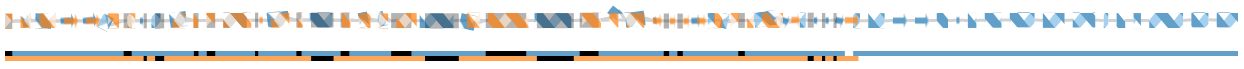
\includegraphics[width=0.9\textwidth]{pics/element.png}
  \caption{Basic element of our proposed visualization consisting of two main parts. The top part shows the secondary structures of the aligned proteins, the bottom part serves for general overview and interactive navigation and selection.}
  \label{fig:element}
\end{figure*}

\subsection*{Design}
The design of the proposed sequential visualization is based on the following requirements:
\begin{itemize}
\item it should convey the information about the constitution of the protein chain wrt. its secondary structures
\item it should serve for multiple comparison of protein chains in represented by its secondary structures
\item the user should be able to easily see the similarities and differences between the chains
\item the user should have the information about the global similarity between proteins 
\item the user should be able to interact with the system in order to explore the similarities and differences in detail
\end{itemize}

Figure~\ref{fig:element} shows the basic element of our proposed visualization.
It demonstrates the case when two proteins chains are aligned.
It consists of two main parts.
The main top part represents the sequential information about protein chain along with its secondary structures.
The bottom part serves for interactive navigation through the protein chain in the top part. 
It informs the user about the length and overall alignment of the compared structures.
Moreover, it enables the user to navigate through the chain and select only an interesting part of the aligned chains, which is then zoomed in the top part.


The interactive navigation part consists of several colored lines where each line corresponds to one protein.
If the protein consists of more chains, the line is interrupted.
Each line can contain black parts which correspond to gaps inserted by the overlay algorithm described in the Implementation section.
These gaps play a role of inserted parts into the straightened chains in order to maintain the correspondence between secondary structures of aligned chains. 
This can happen, e.g., when one chain contains a secondary structure that is missing in the second protein (see Figure~\ref{fig:gap}).
In the top part each gap is represented by gray rectangle.

\begin{figure}[ht]
  \centering
  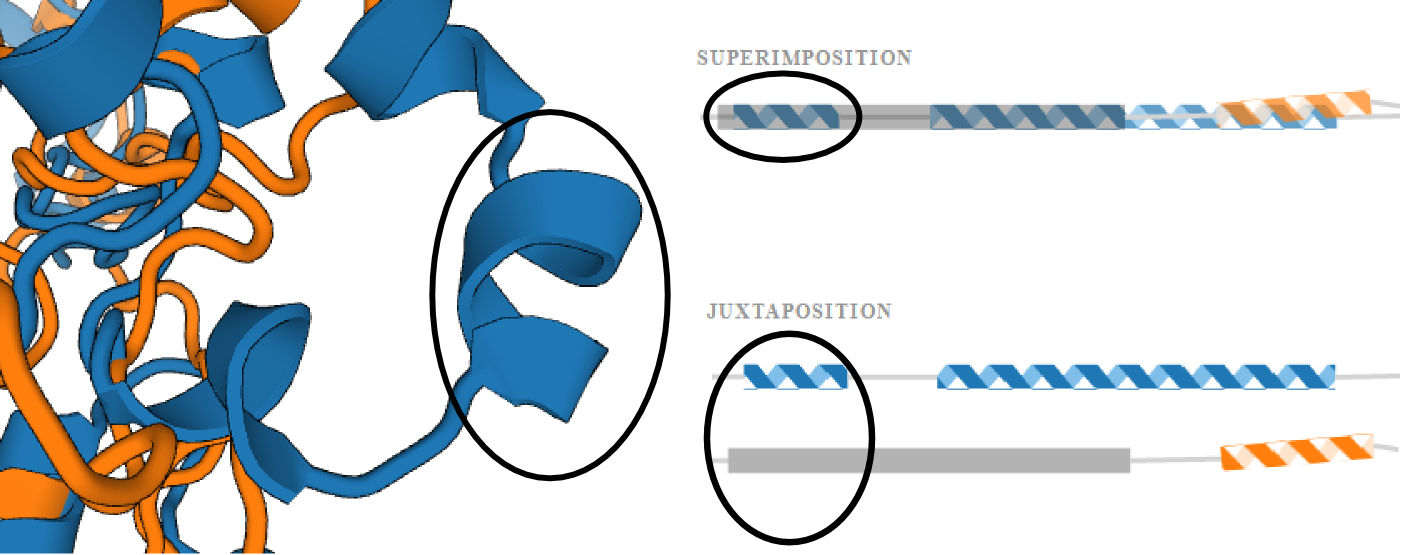
\includegraphics[width=0.9\linewidth]{pics/gap2.png}
  \caption{Example of a helix in the blue protein which does not have its couterpart in the orange protein. This is solved by inserting a gap (gray rectangle) to the superimposed and juxtaposed representations.}
  \label{fig:gap}
\end{figure}

\begin{figure}[th]
  \centering
  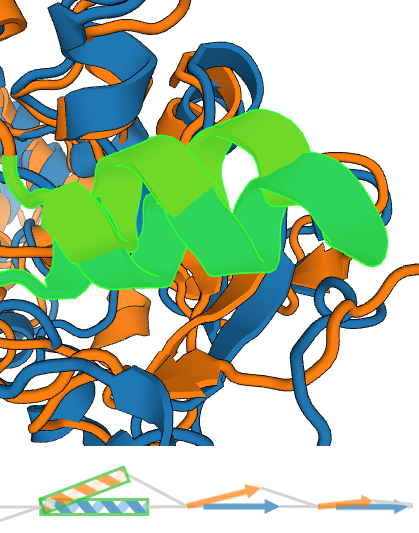
\includegraphics[width=0.9\linewidth]{pics/orientation.png}
  \caption{Example of encoding the mutual orientation of two corresponding helices from the aligned chains (highlighted in green) into our representation. Our visualization maintains the information about the "opening" of the helices.}
  \label{fig:orientation}
\end{figure}

These basic elements are used in two different manners.
In the first case all representations of the aligned chains are superimposed so that the user can immediately see the most similar and different parts of the chains.
The second case shows all aligned chains next to each other which helps to explore individual chains in detail.
In both cases the user can use the navigation slider to select only and interesting part of the chains, zoom in and browse the chain in this zoomed mode.
In the visualization one protein, selected as a reference one, is completely straightened.
The orientation of the secondary structures in the remaining aligned chains is adjusted according to the difference between the position and rotation of the corresponding secondary structures in the reference chain (see Figure~\ref{fig:orientation}).


In consequence, our abstracted representation intuitively navigates the user to the most interesting parts of the chains by linking the selection in the superimposed or juxtaposed view with the 3D representation of the aligned proteins. 

As mentioned before, except for the visualization we proposed also an algorithm for solving the problem of gap insertion.
This is described in detail in the following section.


\subsection*{Implementation}
Our system was implemented using web-based technologies in order to make it available to the wide community of potential users.
Therefore, we used JavaScript along with the D3.js library~\cite{d3} in order to create a fully interactive environment.
Our novel visualization is linked with the 3D representation of the aligned proteins which utilizes the PV viewer~\cite{biasini2014}. 

In the remaining part of this section we describe in detail our proposed algorithms for solving the problems with gap insertion into our visual representation.
We will outline the problem by using a metaphor when the protein chain can be taken as a thread and the secondary structures on this chain will correspond to beads put on this thread.
When comparing more protein chains, we are dealing with a set of threads. 
The beads on these threads can have different colors. 
Their color stands for one secondary structure (helix or strand) which has its unique structure, i.e., consists of a given set of amino acids.
Therefore, the beads with the same color can be positioned on different threads.
In other words, if two beads being on different threads have the same color, it signifies that the corresponding secondary structures were mutually aligned and marked as the corresponding ones. 
Afterward all the threads are arranged below each other.
The task is to position the beads on these threads in such a way that if they correspond to each other (have the same color), they are also positioned below each other. 
The beads can move along the thread but cannot exchange the position with another bead on the same thread.
The following algorithm proposes a simple solution to this problem.

%With the use of the Combinatorial Extension (CE) algorithm for structure alignment~\cite{Shindyalov1998} and force layout algorithm, we let the structures to align in 3D, so there is no deformation caused by choosing a particular projection or distortion. 
%At the end, we visualize the flattened molecules as if they were stretched out from 3D by pulling the chosen reference molecule at its ends into a straight line, so the actual length of secondary structures is preserved as well as the position of near structures of other molecules which are “locked” to the reference molecule.
%Algorithm - GAPS - Detail exploration of differences of two molecules

\subsubsection*{Gap Insertion Algorithm}
\label{sec:alg}
The algorithm for determining the parts on the protein chains where a gap should be inserted works as follows. 
The optimal solution would be to minimize the amount of inserted gaps.
Such solution would be very time and memory consuming.
To overcome this, we propose a greedy algorithm which produces sufficiently correct solution in a fraction of time of the optimal solution.
The correctness was tested on many protein structures and only in some cases our greedy approach inserts a few unnecessary gaps into the chains.

The algorithm operates with pairs of protein chains and it is illustrated in Figure~\ref{fig:alg1}.

\begin{figure}[hbt]
  \centering
  \includegraphics[width=0.9\linewidth]{pics/alg1.png}
  \caption{Principle of the Gap Insertion algorithm. Image illustrates the state when in proteins A and B the helices $i$ and $r$ were already determined as the corresponding ones and the pointers are positioned behind them. Now strand $j$ from A is searched in B and the corresponding strand $t$ is found after skipping one secondary structure. Therefore $n_{gap} = 1$. Similarly, for helix $s$ in B we search for corresponding helix in A. It is the $m$ helix in A and we had to skip 3 secondary structures, so  $m_{gap} = 3$. So we select the first option as the next step, insert one gap to chain A (which will correspond to helix $s$ from B), shift the pointers behind $j$, respectively $t$, and repeat the procedure until both proteins are not processed.}
  \label{fig:alg1}
\end{figure}

The idea for this algorithm comes from the double stack approach when we are able to maintain two stacks in one array.
This is reached by allowing the grow of the stacks in opposite directions.
The algorithm starts by positioning two pointers, each pointer to the beginning of one protein chain.
In each step the algorithm compares the secondary structures from both chains, starting from the pointer positions.
This comparison is performed in two directions, from protein A to protein B and vice versa.
We will describe the principle only for one direction, from A to B.
For the secondary structure at the following position from the pointer of protein A it searches for the corresponding secondary structure in protein B.
The correspondence between the secondary structures is determined from their spatial distance and type.
If found, it counts and remembers the number of secondary structures and their lenghts (lets denote it as $n_{gap}$) which have to be skipped in B to get to the corresponding secondary structure.
The same procedure is performed for protein B, where we obtain $m_{gap}$ as a result.
Then, from these two solutions we take that one which contains less amount of skipped secondary structures.
So if $n_{gap} < m_{gap}$ we insert $n_{gap}$ gaps into protein A, just before the currently processed secondary structure.
The pointer in A is set to this currently processed secondary structure, the pointer in B is shifted to the corresponding secondary structure.
If $m_{gap} < n_{gap}$ we insert $m_{gap}$ gaps into protein B and shift the pointers accordingly.
If $n_{gap}$ or $m_{gap}$ is zero, we do not insert any gap and continue.
The algorithm ends when both protein chains are processed completely.
When one of the chains is already processed and the second chain still contains some remaining secondary structures, we fill the end of the processed chain with gaps.


\subsubsection*{Algorithm for Processing Molecular Dynamics}
When comparing individual time steps of a molecular dynamics simulation, the situation is slightly different. 
We can use the fact that only small changes in its secondary structures and the constitution of the protein chain can occur over time.
%v následující větě jde o jednu AA, nebo o více?
These changes can happen at the ends of the secondary structures where the amino acid can change its membership to the given secondary structure because of the movement of the molecule in the dynamics.
If the secondary structure is very short (consists of one or two amino acids), it can completely disappear in some time steps.
In this specific case we utilize a different approach, illustrated in Figure~\ref{fig:alg2}.

\begin{figure}[hbt]
  \centering
  \includegraphics[width=0.9\linewidth]{pics/alg2.png}
  \caption{Principle of the algorithm processing molecular dynamics. Image illustrates the state when we aim to compare three time steps $A, B, C$ of molecular dynamics simulation. First an artificial chain $A \cup B \cup C$ is created as the union of secondary structures from the thee input chains -- time step. Then each of these chains is compared with the artificial chain using the Gap Insertion algorithm and detected gaps are inserted to the chains.}
  \label{fig:alg2}
\end{figure}

From all time steps we derive one aggregated chain containing all secondary structures which appear at least in one time step. 
In this way we create an artificial chain which is internally stored and not presented to the user.
Then each time step, chain $X$ is compared with this artificial chain and the necessary gaps are inserted into $X$ (here we again utilize our proposed Gap Insertion algorithm).
These gaps are positioned onto the places where the artificial chain contains a secondary structure but chain $X$ does not possess it. 
When all time steps are processed, the artificial chain is removed.


\subsection*{Interaction}
The proposed visualization is directly linked with the 3D view.
The user can interact with both views.
In the 3D view the individual secondary structures are highlighted when hovering over them with mouse and the information about the type and identifier of that secondary structure appears.
When selected by a mouse click, the secondary structure is highlighted in green.
Similarly, the user can select individual secondary structures in the 2D view by clicking on them.
When any of the secondary structures is selected, the highlight of this element is immediately projected to the second view.
This functionality gives the user an insight on the spatial positions of the selected structures.
It also offers independent interaction with both views yet still in context of the selected elements.

We also provide the users with a configuration panel located below the 3D view which allows the user to load individual structures and further manipulate with them, e.g., defining the reference protein onto which the remaining proteins are aligned.
Proteins in the juxtaposition view are by default sorted by the computed RMSD between the reference protein and the others.
Therefore, the most similar proteins are positioned closer to the reference protein on the top.
However, this order can be changed by simple interaction with the user interface.   

\section*{Results and Discussion}
Our proposed visualization was tested on several case studies proposed by the biochemists.
Here we will describe two selected cases.
The first study compares six proteins from the cytochrome P450 family of proteins which are published and compared in the review paper by Cojocaru et al.~\cite{Cojocaru2007}. 
The authors present newly revealed channels in this family of proteins.
Studying these channels is of high interest because they can serve for transportation of ligands to the protein active site where a chemical reaction between the protein and ligand can occur.
The study demonstrates how some of the channels can merge when the protein structures change.
This merge is largely caused by movements of specific secondary structures.
These movements are most significant when comparing crystal structures of the mammalian and bacterial enzymes.

The authors are exploring six enzymes (with PDB identifiers 2D09, 1JPZ, 1PQ2, 1IZO, 1F4T, and 1NR6) which represent different topologies of cytochrome P450. 
The presence and position of channels in these enzymes are distinguished by the secondary structure elements lining the channels at the protein surface. 
As the positioning of the secondary structures varies from one cytochrome to another, the spatial location of channels vary considerably as well.
Therefore, the key to understand the differences between channels lies in the exploration of changes between the spatial positions of lining secondary structures.
However, using the juxtaposed views illustrated in the paper or superimposing the 3D representations it is very hard to reveal the differences in positions of the secondary structures (see Figure~\ref{fig:many}).

Using our newly proposed representation the user can immediately see the differences in the aligned chains of these structures (see Figure TODO).
By selecting those interesting parts in the 2D view the user is intuitively navigated to the areas in 3D space where these parts are located.
This enables fast exploration of the aligned chains and changes in the void space lined by the secondary structures which determines the geometric properties of channels.

The second study focuses on the exploration of protein flexibility.
This can be reached by studying the behavior of the protein via the molecular dynamics simulations.
Individual secondary structures of the protein can change their positions over time and the the more significant movement, the more flexible a given secondary structure is.
Therefore, we can study the protein behavior by comparing the protein chain in selected time steps.
Here our representation again helps to reveal the most similar (i.e., stable) and most different (i.e., flexible) secondary structures (see Figure TODO) and to navigate the user to these parts in the 3D view.

The domain experts concluded that our proposed 2D representation along with its integrated 3D view is innovative because it helps them to easily reveal the most interesting parts of the aligned protein chains.
Thus, it overcomes the occlusion problems because the user is directly navigated only to the specific parts of the chains in the 3D view.

\section*{Conclusions}
In this paper we proposed a novel visual representation of protein chains which helps to intuitively compare several aligned protein chains and to reveal their most significant parts.
The representation uses combines the advantages of the 2D sequential representation and 3D view and help the user to understand the mutual position of secondary structures in the aligned chains and explore them in 3D.
The usability of our approach was tested on several case studies and the domain experts confirmed that it helped them to reveal and understand the differences between secondary structure positions more quickly and intuitively than before.

Our representation can be further improved in several ways. 
One bottleneck of our approach currently lies in the Gap Insertion algorithm which, due to its simplicity, can in some specific cases insert too much gaps.
Therefore, we will design and implement more sophisticated, yet time and memory efficient, approach to visualizing gaps in superimposition of more than two structures.
Another possible extension, also suggested by the domain experts, was to automatically highlight interesting parts of the chains by introducing a similarity index.
Of course, this index has to be defined in tight cooperation with the biochemists.
When comparing many proteins or many time steps, the visualization starts to be too complex.
In these cases the user is mostly interested in the most differences between the chains.
Therefore, we could implement a contour-based visualization which outlines only the contours of the superimposed structures.
Finally, our representation could be further equipped with the additional information about positions of protein channels, interacting ligands, and other biochemically relevant structures.

%%%%%%%%%%%%%%%%%%%%%%%%%%%%%%%%%%%%%%%%%%%%%% 
%%                                          %%
%% Backmatter begins here                   %%
%%                                          %%
%%%%%%%%%%%%%%%%%%%%%%%%%%%%%%%%%%%%%%%%%%%%%%

\begin{backmatter}

%\section*{List of abbreviations used}
%TIM: \textit{triosephosphate isomerase}, scTIM: \textit{saccharomyces
%cerevisiae triosephosphate isomerase}, dTIM: \textit{defective triosephosphate
%isomerase}, PDB: \textit{protein data bank}.

\section*{Competing interests}
The authors declare that they have no competing interests.


%%%%%%%%%%%%%%%%%%%%%%%%%%%%%%%%%%%%%%%%%%%%%%%%%%%%%%%%%%%%%
%%                  The Bibliography                       %%
%%                                                         %%
%%  Bmc_mathpys.bst  will be used to                       %%
%%  create a .BBL file for submission.                     %%
%%  After submission of the .TEX file,                     %%
%%  you will be prompted to submit your .BBL file.         %%
%%                                                         %%
%%                                                         %%
%%  Note that the displayed Bibliography will not          %%
%%  necessarily be rendered by Latex exactly as specified  %%
%%  in the online Instructions for Authors.                %%
%%                                                         %%
%%%%%%%%%%%%%%%%%%%%%%%%%%%%%%%%%%%%%%%%%%%%%%%%%%%%%%%%%%%%%

% if your bibliography is in bibtex format, use those commands:
\bibliographystyle{bmc-mathphys} % Style BST file
\bibliography{bmc_article}      % Bibliography file (usually '*.bib' )

% or include bibliography directly:
% \begin{thebibliography}
% \bibitem{b1}
% \end{thebibliography}

%%%%%%%%%%%%%%%%%%%%%%%%%%%%%%%%%%%
%%                               %%
%% Figures                       %%
%%                               %%
%% NB: this is for captions and  %%
%% Titles. All graphics must be  %%
%% submitted separately and NOT  %%
%% included in the Tex document  %%
%%                               %%
%%%%%%%%%%%%%%%%%%%%%%%%%%%%%%%%%%%

%%
%% Do not use \listoffigures as most will included as separate files

%\section*{Figures}
%  \begin{figure}[h!]
 % \caption{\csentence{Sample figure title.}
  %    A short description of the figure content
   %   should go here.}
   %   \end{figure}

%\begin{figure}[h!]
 % \caption{\csentence{Sample figure title.}
  %    Figure legend text.}
  %    \end{figure}

%%%%%%%%%%%%%%%%%%%%%%%%%%%%%%%%%%%
%%                               %%
%% Tables                        %%
%%                               %%
%%%%%%%%%%%%%%%%%%%%%%%%%%%%%%%%%%%

%% Use of \listoftables is discouraged.
%%
%\section*{Tables}
%\begin{table}[h!]
%\caption{Sample table title. This is where the description of the table should go.}
 %     \begin{tabular}{cccc}
%        \hline
 %          & B1  &B2   & B3\\ \hline
 %       A1 & 0.1 & 0.2 & 0.3\\
 %       A2 & ... & ..  & .\\
 %       A3 & ..  & .   & .\\ \hline
 %     \end{tabular}
%\end{table}

%%%%%%%%%%%%%%%%%%%%%%%%%%%%%%%%%%%
%%                               %%
%% Additional Files              %%
%%                               %%
%%%%%%%%%%%%%%%%%%%%%%%%%%%%%%%%%%%

%\section*{Additional Files}
%  \subsection*{Additional file 1 --- Sample additional file title}
%    Additional file descriptions text (including details of how to
%    view the file, if it is in a non-standard format or the file extension).  This might
%    refer to a multi-page table or a figure.

%  \subsection*{Additional file 2 --- Sample additional file title}
%    Additional file descriptions text.

\end{backmatter}
\end{document}
